\chapter{Was ist Testmanagement?}
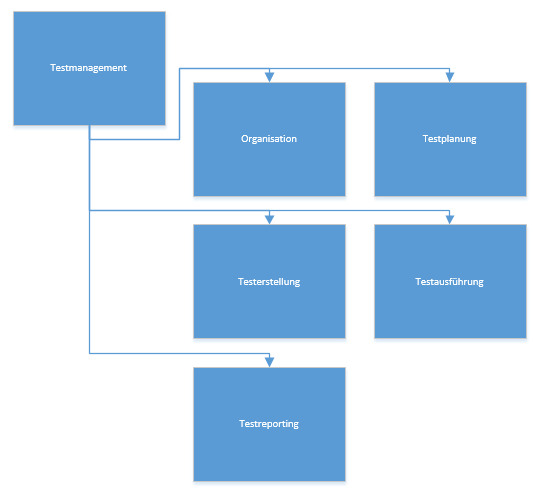
\includegraphics[]{images/testmanagement}
\section{Organisation}
Ein notwendiger Teil des Testmanagements ist die Organisation von Resourcen und Testartefakten. Hierbei geht es quasi darum die Basis f\"ur alles weitere zu erstellen. 

\section{Testplanung}
Die Testplanung besch\"aftigt sich mit den Fragen \textit{Was?}, \textit{Wann?}, \textit{Wo?} und \textit{Wieso?} getestet wird.

\begin{itemize}
	\item \textit{Wieso?} - Der Grund f\"ur einen Test ist beispielsweise eine Anforderung, die validiert werden muss.
	\item \textit{Was?} - Was getestet wird ergibt aus den Anforderungen. 
	\item \textit{Wo?} - Der Ort des Tests h\"angt von den Software- und Hardwareanforderungen ab
	\item \textit{Wann?} - Wann getestet wird ergibt sich aus den Entwicklungszyklen.
\end{itemize}


\section{Testerstellung}
Bei der Testerstellung werden die n\"otigen Schritte eines Tests definiert.  

\section{Testausf\"uhrung}
Bei diesem Teil geht es darum fest zu legen wie getestet wird. Im speziellen werden hier aus einzelnen Testf\"allen sogenannte Testsuites(eine Abfolge von Tests) erstellt.

\section{Testreporting}
Das Testreporting besch\"aftigt sich mit der Analyse und der Dokumentation der Testergebnisse.

\chapter{Ziele}
\section{Qualit\"atssteigerung}
Das Wohl offensichtlichste Ziel des Testmanagements ist die Qualit\"atsteigerung. Durch gutes Testmanagement k\"onnen fehler fr\"uhzeitig gefunden und behoben werden. Eine h\"ohere Qualit\"at an Testf\"allen bringt meist mehr Fehler zu tage. Je mehr Fehler gefunden werden desto mehr Fehler k\"onnen auch behoben werden. Je besser die Fehler dokumentiert sind desto besser k\"onnen sie nach vollzogen und damit auch behoben werden.

\section{Hohe Testabdeckung}
Gutes Testmanagement schont die Resource Zeit wodurch mehr getestet werden kann, was wiederum die Testabdeckung steigert. Zudem kann beispielsweise durch Testautomatisierung die Testabdeckung deutlich gesteigert werden.

Auch schon in fr\"uheren Schritten, etwa im Schritt der Testplanung, kann hierf\"ur einiges an Vorarbeit geleistet werden. Entsteht durch eine schlechte Planung eine schlechte Testabdeckung(z.b.: es werden einige Anforderungen ausgelassen), so kann diese sp\"ater nur schwer korrigiert werden. 

\section{Kostensenkung}
Auch eine Senkung der Kosten kann aus gutem Testmanagement resultieren. Hierbei schlie\ss{}t sich nicht wie \"ublich eine Sekung der Kosten und eine Steigerung der Qualit\"at aus. Oftmals gehen diese miteinander ein. Ein gutes Beispiel hierf\"ur ist die Testautomatisierung.

\section{Dokumentation}
Nat\"urlich ist auch die Dokumentation der Tests und deren Ergebnisse wichtig. F\"ur eine gute Dokumentation gibt es viele Gr\"unde. Man kann dem Kunden gegen\"uber zeigen mit welchen Mitteln man f\"ur die gew\"unschte Qualit\"at des Produktes sorgt. Man hat aber auch einen besseren \"Uberblick bei anstehenden Entscheidungen. Nicht zu letzt sammelt man so auch gut dokumentierte Erfahrungswerte, die f\"ur weitere Projekte hilfreich sein k\"onnen.

\chapter{Herausforderungen}
\section{Nicht genug Zeit zum Testen}
Zeit ist in der Regel ohnehin ein kritischer Faktor bei der Softwaeentwicklung. Wird die Zeit knapp, so wird meist bei der Zeit zum Testen gespart. Kommt es dann noch zu Verz\"ogerungen bei der Implementierung, so kann es durchaus sein, dass die fehlende Zeit beim Testen weg genommen wird.

\section{Nicht genug Resourcen zum Testen}
Oftmals ist es ein Problem die ben\"otigten Resourcen zum durchf\"uhren der Tests zu bekommen. Nicht nur Hardware-Resourcen k\"onnen hierbei ein Problem darstellen. Mitarbeiter, die die Tests durchf\"uhren sollen, k\"onnen ein noch gr\"o\ss{}eres Problem darstellen.

\section{R\"aumlich getrennte Teams}
R\"aumliche Trennung der Teams kann auch zu einem Problem werden. Wenn sich das Entwicklungsteam und das Teastteam beispielsweise auf verschiedenen Kontinenten mit verschiedenen Zeitzonen befinden. Dies ist durchaus g\"angig bringt allerdings technische Hindernisse mit sich. Wie werden Artefakte unter den Teams geteilt? Wie schaffen es die Teams ohne Verz\"ogerungen kordiniert zu bleiben? Wie knn die Projekteffizienze hierdurch gesteigert werden?

\section{Probleme mit Anforderungen}
Die Anforderungen zu validieren ist in der Regel die Hauptstrategie beim Testen. Damit dies auch funktionieren kann m\"ussen die Anforderungen auch testbar und vollst\"andig sein. Es muss jederzeit Zugriff auf die aktuellen Anforderungen und dem dazu geh\"origen System geben. 

\section{Die richtigen Informationen berichten}
Tests sind nur dann n\"utzlich, wenn sie den Status der Entwicklung und deren Qualit\"at zeigen k\"onnen. Die Testergebnisse passend f\"ur alle relevante Personen zur rechten Zeit bereit zu stellen kann sich als echte Herausforderung herausstellen. 

Hierf\"ur gibt es mehrere Gr\"unde:
\begin{itemize}
	\item \textbf{Zu wenig Informationen} k\"onnen einem zu schlechten \"Uberblick \"uber das Projekt f\"uhren
	\item \textbf{Zu viele Informetionen} k\"onnen den eigentlichen Grund des Tests verdecken
\end{itemize}

Die Art der Darstellung der Ergebnisse ist auch ein wichtiger Punkt. Unabh\"angig von der Art der Darstellung(dokumentbasiert, browserbasiert, toolbasiert, etc.) ist es wichtig die Daten klar und logisch darzustellen.

\section{Welche Qualit\"atsmetriken werden verwendet?}
Eines der Zeile des Testens ist es die Quali\"at darzustellen. Hierzu m\"ussen die verwendeten Qualit\"atsmetriken festgelegt werden. Hierbei gilt im Allgemeinen, dass die Metriken so komplex wie n\"otig, aber so simpel wie m\"oglich sein sollen.

\chapter{Testmanagementtools}
Testmanagementtools sind ein wichtiges Werkzeug das Testmanagement zu unterst\"utzen. Diese Tools sind unverzichtbar f\"ur ein erfolgreiches Testmanagement und damit auch f\"ur eine erfolgreiche Softwareentwicklung.

\section{Beispiele}
Im folgenden werden einige Beispiele kurz erl\"autert.

\subsection{HP Quality Center}
Das HP Quality Center ist eine recht komplexe, kostenflichtige L\"osung. Das HP Quality Center deckt einen gro\ss{}en Teil des Testmanagements ab. Es bietet beispielsweise die M\"oglichkeit Testf\"alle aufzuzeichnen und anschlie\ss{}end f\"ur die Automatisierung bereit zu stellen.

\subsection{Testlink}
Testlink ist ein Tool zur Verwaltung und Erstellung von Testf\"allen, Testsuites und Testergebnissen. 

\subsection{IBM Rational Quality Manager}
Auch von IBM gibt es ein Testmanagementtool. Sie bietet \"ahnliche Optionen wie das HP Quality Center.

\subsection{Redmine}
Redmine ist eine webbasierte L\"osung, die das Tracking von Aufgaben, Features und Bugs besch\"aftigt. Redmine l\"a\ss{}t sich \"uber Plugins erweitern um beispielsweise Scrum zu unterst\"utzen.

\section{Kosten und Nutzen}
\subsection{Nutzen}
\begin{itemize}
	\item Standardisierung der Dokumentation: Eine standardisierte Dokumentation macht es leichter den Verlauf zu verfolgen, Ergebnisse zu bewerten, etc.
	\item Verfolgbarkeit der Testartefakte: Man kann schnell und direkt den Status von Testartefakten abfragen.
	\item Flexibilisierung der Testprozesse: Unter zu Hilfenahme von Tools k\"onnen beispielsweise Testsuites schnell und flexibel den wechselnden Anforderungen und H\"urden angepasst werden.
	\item Optimierung/Verk\"urzung des kritischen Pfads: Die Verwendung von Testmanagementtools steigert im Allgemeinen die Geschwindigkeit in des gesammten Testprozesses. Blockiert nun ein Testdurchlauf die Entwicklung wirkt sich diese Steigerung als eine Verk\"urzung des kritischen Pfades aus.
\end{itemize}
\subsection{Kosten}
\begin{itemize}
	\item Lizenzen: Bei den Tools mit gr\"o\ss{}erem Umfang fallen oftmals Anschaffungskosten und sogar Lizenzkosten an. Diese sind teilweise nicht unerheblich.
	\item Betrieb: Auch der Betrieb solcher Tools kostet Geld, beispielsweise durch deren Wartung.
	\item Training: Je mehr die Tools leisten k\"onnen desto mehr Training muss in die Benutzer investiert werden.
\end{itemize}

\chapter{Empfehlungen}
\section{Starte Testaktivit\"aten fr\"uhzeitig}
Auch wenn diese Empfehlung sehr offensichtlich ist wird sie dennoch von den wenigstens Projekten wirklich beachtet. Tests s fr\"uh wie m\"oglich durchzuf\"uhren kann viele Probleme bereits fr\"uhzeitig aufdecken. Zudem k\"onnen hierdurch zeitliche Probleme minimiert werden.

\section{Iterative Tests}
Iterative Tests helfen fr\"uhzeitig Testergebnisse zu liefern.

\section{Wiederverwendung von Testartefakten}
Durch die Wiederverwendung von Testartefakten kann nicht nur Zeit gespart werden. Es k\"onnen auch Resourcen gespart werden. Gerade Dinge wie das Einrichten eines Testsystems kosten oftmals viel Zeit und auch Resourcen. In vielen F\"allen kann man des Testsystem aber f\"ur viele verschiedene Tests und auch verschiedene Testiterationen verwenden.

Die Wiederverwendbarkeit beschr\"ankt sich hierbei nicht auf ein Projekt. Oftmals sind Testsysteme f\"ur mehrere Projekte n\"utzlich. 

Die Wiederverwendung beschr\"ankt sich hierbei aber nicht auf Testsysteme. Es k\"onnen auch Testprozesse wieder verwendet werden.

Damit dies auch funktioniert muss das Testmanagement gut organisieren. Damit Artefakte wiederverwendet werden k\"onnen muss vorausschauend geplant werden wenn Artefakte erstellt werden.

\section{Verwende Tests basierend auf Anforderungen}
Testen kann in zwei Herangehensweisen unterteilt werden:
\begin{itemize}
	\item Validieren dass etwas macht was es soll
	\item Versuchen herauszufinden wie man etwas kaputt macht
\end{itemize}

Der zweite Punkt ist mit Sicherheit nicht unwichtig und hilft gerade bei schwer absehbaren Szenarien Fehler zu finden, allerdings ist das Validieren der Anforderungen der wohl kritischte Punkt.

Beim Validieren der Anforderungen kann eine bessere Absch\"atzung des zeitlichen Aufwandes gegeben werden. Dies erleichtert die Planung des Testvorg\"ange.

Zudem kann es auch Statistiken, wie beispielsweise Testabdeckung, liefern.

Das Erstellen von Testf\"allen anhand von Anforderungen und das Festhalten der Beziehung kann zu einer komplexen Aufgabe werden. Daher empfiehlt es sich dies unter zu Hilfe nahme eines Tools zu machen.

Nat\"urlich ist es hierf\"ur erforderlich, dass die Anforderungen eindeutig und klar formuliert sind. Je weniger Subjektivit\"at in die Testf\"alle einflie\ss{}t desto besser. Damit h\"angt dieses Verfahren stark von anderen Teilen des Entwicklunsgprozesses ab.

Am effektivsten ist eine Mischung von verschiedenen Herangehensweisen. Das Validieren der Anforderungen sollte allerdings immer ein fester Bestandteil des Testmanagements sein.

\section{Nutze entfernte Testresourcen}
Um Resourcenmangel entgegen zu wirken kann es n\"utzlich sein auf entfernte Resourcen zur\"uck zu greifen. Dies bringt nat\"urlich neue Herausforderungen mit sich. Entfernte Resourcen m\"ussen koordiniert werden, damit sie einen Vorteil bringen.

\section{Rest der Entwicklung mit einbeziehen}
Auch wenn es im Normalfall besser ist unbefangene Tester zu haben, die m\"oglichst nichts von dem zu testenden System wissen sollte dies keine Barriere zwischen Testern und Entwicklern erzeugen. Unter anderem ist die Kommunikation zwischen Testern und Entwicklern wichtig. Auch an dieser Stelle stellt die Verwendung von Tools einen gro\ss{}en Vorteil dar. Dies reicht von den Erstellen vin Bugs in einem Bug-Tracking-Tool(dem Festhalten des Fehlers) zu der M\"oglichkeit ohne gro\ss{}en Aufwand eine gezielte und direkte Kommunikation zwischen Bug-Ersteller und verantwortlichem Entwickler zu sichern. Es ist also wichtig diese Grenze nicht als Blockade anzusehen.

\section{Kommuniziere den Status}
Jeder Test ist nur so wertvoll wie die Informationen \"uber ihn die mitgeteilt werden. Daher ist es wichtig, dass Testreports vollst\"andig sind. Desweiteren ist es wichtig, dass die Art in der die Information weitergegeben wird dem Zweck entspricht.

Beim Reporting ist es wichtig nicht starr bereits vorhandene Dokumente zu verwenden, sondern bei Bedarf diese auch anzupassen oder gar komplett neu zu erstellen. Nat\"urlich stellt dies einen Mehraufwand dar, aber dieser Mehraufwand sollte f\"ur die bessere Qualit\"at der Testreports in Kauf genommen werden.

Testreports sind oft eine Entscheidungsgrundlage oder tragen wenigstens zu Entscheidungen bei, daher ist es unmso wichtiger, dass deren Qualit\"at m\"oglichst hoch ist. Was bringen die besten Tests, wenn die Testreports die Ergebnise nicht klar genug darstellen?

\section{Ziele und Ergebnise fokusieren}
Ein wichtiger Punkt beim Testmanagement ist es die Ziele im Bereich der Qualit\"at im Auge zu behalten und wie man diese effektiv und akkurat misst. Die Aufabe des Testmanagements ist es eben dies zu definieren.

Nicht alle Aufgaben haben offensichtliche Erf\"ullungskriterien. Durch das Definieren dessen, was eine Aufgabe liefern soll und das Festlegen der Metriken f\"ur die Bewertung der Tests macht es leichter den Status der Aufgabe zu beobachten.

Wichtig ist es auch im Bereich des Testens eine Versionierung zu verwenden. Dies schlie\ss{}t die Ergebnisse der Tests mit ein. Hierdurch hat man zu jeder Zeit einen \"Uberblick \"uber die Entwicklung des Systems und kann helfen Entscheidungen zu treffen.

\section{Automatisierung}
Wie es so oft der Fall ist ist Zeit meistens die knappste Resource. Hier kann Automatisierung Abhilfe schaffen. Grunds\"atzlich ist Automatisierung immer dann zu empfehlen, wenn ein Test oft durchgef\"uhrt wird. Bei einmaligen Tests macht eine Automatisierung im Allgemeinen keinen Sinn. Ausnahmen w\"aren Tests bei denen beispielsweise die selbe Aktion mit vielen verschiedenen Werten durchgef\"uhrt wird, wobei dies im Grunde ein mehrfaches Aufh\"uhren des Tests ist. Gerade bei Iterativer Entwicklung helfen automatisierte Tests. Testdriven Development stellt diese in den Vordergrund.

Automatische Tests verbrauchen keine menschlichen Resourcen(nach deren Erstellung) und eignen sich wunderbar um beispielsweise \"uber Nacht oder \"uber das Wochenende durchgef\"uhrt zu werden. Man kann so beispielsweise erreichen, dass man an jedem Morgen einen aktuellen \"Uberblick \"uber den Stand des Sytems hat.

Man sollte sich allerdings immer vor der Automatisierung \"uberlegen ob es sich zeitlich lohnt. Wenn das Erstellen des automatischen Testfalls den Zeitaufwand f\"ur das manuelle Durchf\"uhren \"uberschreitet k\"onnte dies ein Grund sein, der gegen eine Testautomatisierung spricht. Da sich die Softwareentwicklung immer mehr in die agile Richtung entwicklet wird Testautomatisierung immer wichtiger.
